

%%!TEX encoding = UTF-8 Unicode 
%\documentclass[compress, gray]{beamer}
\PassOptionsToPackage{table}{xcolor}
\documentclass[yellow]{beamer}
\mode<presentation>
%\usetheme{Singapore}
\usetheme{Szeged}
%\usetheme{Warsaw}
%\usetheme{Antibes}
%\usecolortheme{lily}
\usecolortheme{orchid}
%\useoutertheme[subsection=false]{smoothbars}
\useoutertheme[subsection=true]{smoothbars}
%\useoutertheme[subsection=true]{shadow}
%\useoutertheme{smoothbars}
%\useinnertheme{circles}
\useinnertheme{rounded} 
%\useinnertheme{rectangles}
%\beamertemplateballitem

\usepackage{lmodern}
\usepackage[brazil]{babel}
\usepackage[utf8]{inputenc}
\usepackage[ruled,vlined]{algorithm2e}
\usepackage{listings}
\usepackage{graphicx,url}
\usepackage{listings}
\usepackage{url}

%\usepackage[table]{xcolor}

\renewcommand{\lstlistingname}{Listagem}


\title{ChessPhi}

\author{\underline{Alexandre Brisighello \& Marcus Botacin}}


%\date{5 de Novembro de 2014 } 

\begin{document}

\frame{
	\titlepage
}

\AtBeginSubsection[]
{
	\begin{frame}<beamer>
		\frametitle{Tópicos}
		\tableofcontents[currentsection,currentsubsection]
	\end{frame}
}

\begin{frame}
 \frametitle{Tópicos}
 \tableofcontents
%   You might wish to add the option [pausesections]
\end{frame}

\section{Implementação}

%\subsection{ChessPhi}

\begin{frame}
  \frametitle{Requisitos e Objetivos}

\begin{itemize}
\item Jogo de Xadrez
\item Xeon Phi
\item \textit{Alfa Beta Prunning}
\item \textit{Bag of Tasks}
\end{itemize}
\end{frame}

\begin{frame}
  \frametitle{Min-Max}
  \begin{figure}[!hpbt]
	  \centering
	  \begin{minipage}{1\textwidth}
		    \centering
		      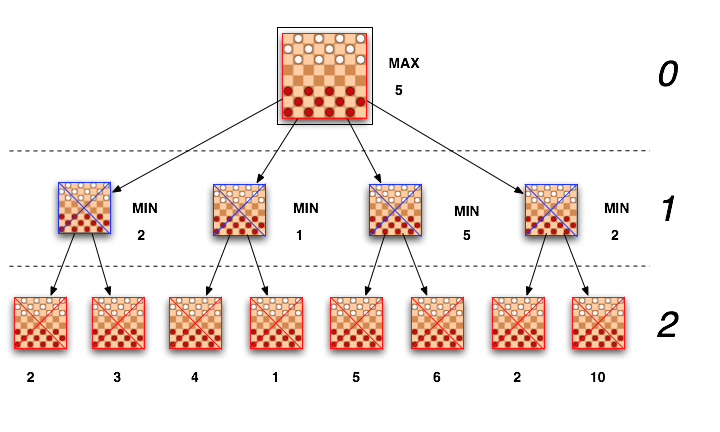
\includegraphics[width=.8\linewidth]{minimax.png}
		        \caption{Exemplo}{Min-Max}
			  \label{fig:1}
		  \end{minipage}
	  \end{figure}
  \end{frame}

\begin{frame}
  \frametitle{Alfa-Beta}
  \begin{figure}[!hpbt]
	  \centering
	  \begin{minipage}{1\textwidth}
		    \centering
		      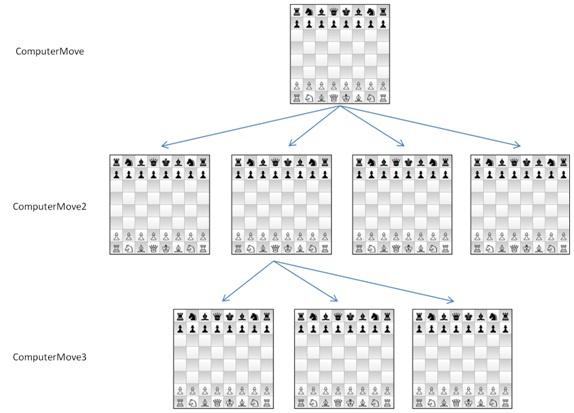
\includegraphics[width=.8\linewidth]{huoChess_2.jpg}
		        \caption{Exemplo}{Alfa-Beta}
			  \label{fig:1}
		  \end{minipage}
	  \end{figure}
  \end{frame}


\section{Resultados}


\begin{frame}
	\frametitle{\textit{Benchmarks}}
\end{frame}

\end{document}
